\chapter{Grundlegende Verfahren der semantischen Segmentierung}

Ziel der semantischen Segmentierung von 3D-Daten ist es, jedem Punkt im Raum
einer bestimmten Kategorie zuzuordnen und dadurch Bereiche des Bildes in
klassifizierte Objekte zu unterteilen. Hierfür gibt es verschiedene Ansätze,
die auf Erweiterungen von neuronalen Netzen basieren.

\section{Convolutional Neural Networks (CNNs)}
Convolutional Neural Networks (CNNs) sind eine erweiterte Art von künstlichen
neuronalen Netzen, die speziell für die Verarbeitung von Bildern entwickelt
wurden. Sie bestehen aus mehreren Schichten, darunter Convolutional Layers,
Pooling Layers und Fully Connected Layers, die miteinander verbunden sind. Die
Architektur der CNNs ist dabei nicht vorgegeben, folgt aber in der Praxis immer
einer ähnlichen Vorlage. Ein beispielhafter Aufbau ist in Abbildung
\ref{fig:CNN} dargestellt. Der Input-Layer beinhaltet die Pixelwerte des
Bildes. Darauf folgen in der Regel ein oder zwei Convolutional-Layers,
woraufhin sich ein Pooling-Layer anreiht. Die Kombination aus Convolutional-
und Pooling-Layer kann dabei je nach Komplexität beliebig oft im Netz
vorkommen. Am Ende folgt ein Fully-Connected-Layer an den der Output anknüpft.
Dieser gibt das Klassifizierungsergebnis des betrachteten Bildes durch das
Netzwerk aus. Die Convolutional-Layers können vereinfacht als Filter-Layer
betrachtet werden und extrahieren markante Merkmale aus den Eingabebildern, um
die Klassifikation zu erleichtern. Dabei wird jeder Bereich des Bildes pro
Layer mit einem Kernel gefaltet und erzeugen eine 2D-Aktivierungskarte. Die
Kernels besitzen dabei häufig kleine räumliche Dimensionalität, erstrecken
sich aber über die gesamte Tiefe des Eingangsbildes. Die Anschließend folgenden
Pooling-Layers dienen dazu, die Dimensionen der Ausgabe des
Convolutional-Layers zu reduzieren und somit die Rechnenkomplexität des Modells
zu verringern. Besonders häufig kommen dabei sogenannte Max-Pooling-Layers zum
Einsatz. Bei diesen wird ein Kernel einer beliebigen Größe, ohne zu überlappen,
über die Aktivierungskarte geschoben. Dabei wird nur der größte
Aktivierungswert eines Fensterbereiches übernommen und so die Dimensionalität
der Aktivierungskarte stark reduziert. Darauf folgt häufig ein Flatten-Layer,
der die Aktivierungskarte in einen eindimensionalen Raum überführt, welcher von
den nachfolgenden Fully-Connected-Layers verarbeitet werden kann. Die Fully
Connected Layers am Ende des Netzes verarbeiten schließlich die extrahierten
Aktivierungen und versuchen daraus Klassifizierungsergebnisse zu gewinnen. Der
Hauptanwendungsbereich von CNNs liegt dabei in der Klassifikation von Bildern
in vorbestimmte Kategorien. \cite{11262015}.

\begin{figure}[h]
    \centering
    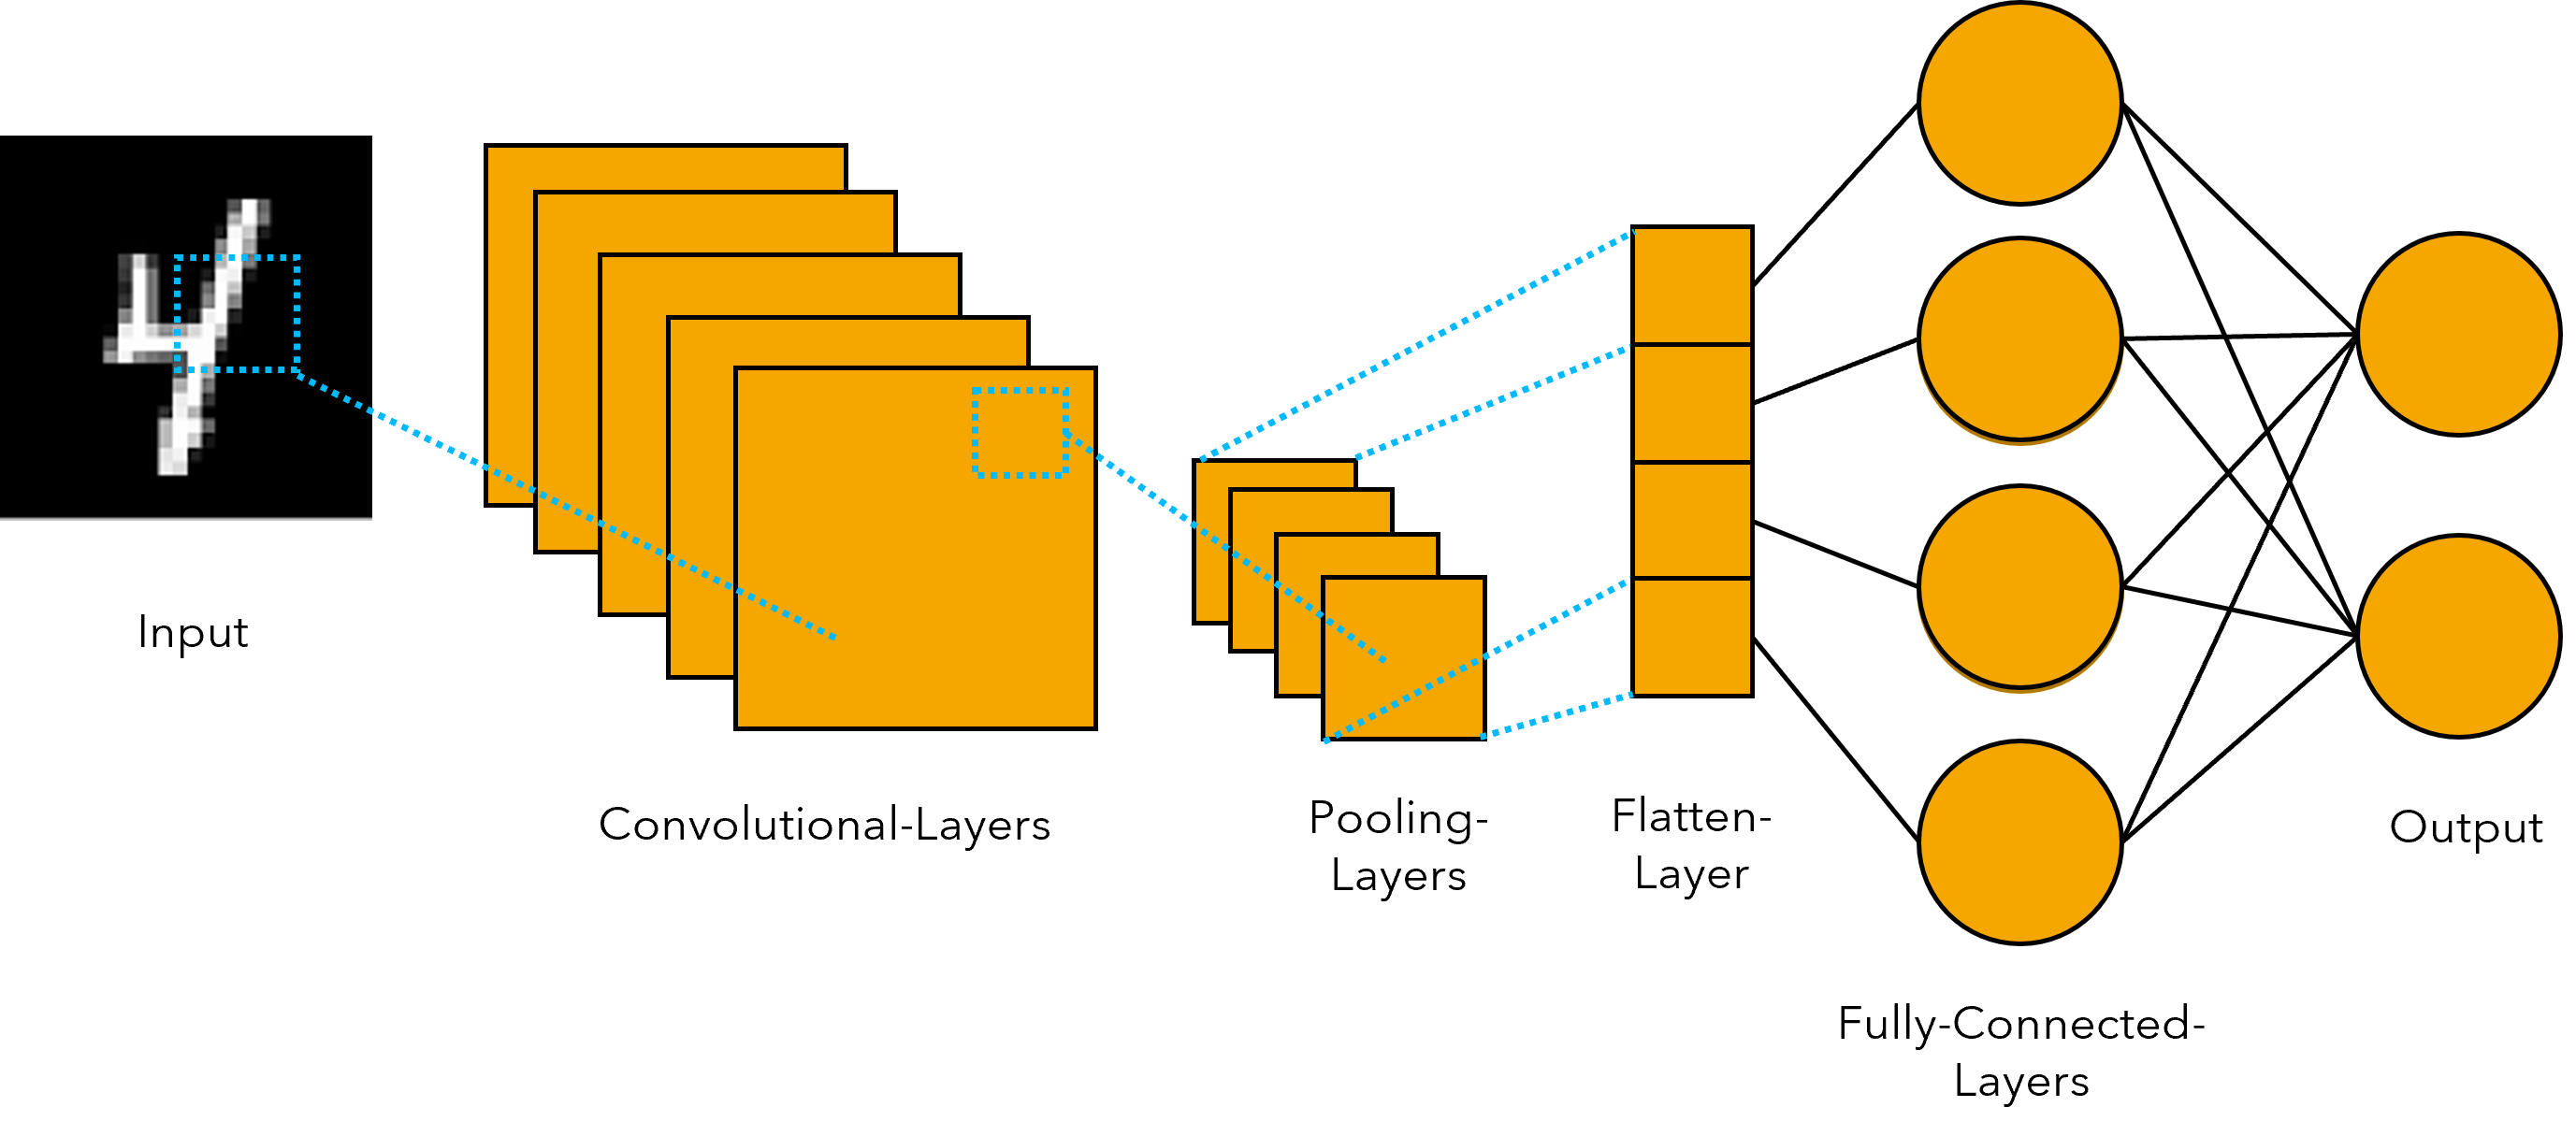
\includegraphics[width=1\textwidth]{bilder/cnn_own.png}
    \captionsetup{font=small} % Hier die gewünschte Größe einstellen
    \caption[Aufbau eines Convolutional Neural Networks, beispielhaft mit dem Modified National
    Institute of Standards and Technology Datensatz (MNIST-Datensatz)]{Aufbau eines Convolutional Neural Networks, beispielhaft mit dem Modified National
        Institute of Standards and Technology Datensatz (MNIST-Datensatz), Ähnlich \cite{jalandoni2022use}}
    \label{fig:CNN}
\end{figure}

\section{Fully Convolutional Networks (FCNs)}
Fully Convolutional Networks (FCNs) sind eine Weiterentwicklung von CNNs, die
speziell für die Aufgabe der semantischen Segmentierung von Bildern entwickelt
wurden. Im Gegensatz zu herkömmlichen CNNs, die für die Klassifizierung und
Erkennung von Objekten in Bildern ausgelegt sind, können FCNs jedes Pixel eines
Eingabebildes klassifizieren und somit die räumlichen Informationen der
klassifizierten Bilder beibehalten. FCNs verwenden dabei ausschließlich
Convolutional-Layers und Pooling-Layers, nicht aber Fully-Connected-Layers.
Dies ermöglicht es eine Merkmalskarte des Eingabebildes zu erzeugen, auf der
jedes Pixel einer bestimmten Klasse zugeordnet wird. Durch die Verwendung von
FCNs können somit komplizierte Zusammenhänge innerhalb von Bildern auf der
Ebene der Pixel identifiziert werden, was für Anwendungen wie die autonome
Navigation oder Objekterkennung von großer Bedeutung ist. \cite{7803544}
Bekannte und erfolgreiche Verfahren, wie das U-Net, verwenden dabei häufig eine
Encode-Decoder-Architektur, um das Klassifizierungsergebnis in der
Dimensionalität des Eingangsbildes darzustellen \cite{8309343}.

\section{Encoder-Decoder-Architekturen}
Encoder-Decoder-Architekturen stellen eine spezielle Architektur von neuronalen
Netzen dar. Der Name leitet sich aus deren Aufbau ab, welcher aus zwei
Hauptkomponenten, einem Encoder und einem Decoder, besteht. Der Encoder
verwendet typischerweise Convolutional und Pooling-Layers, um das Eingabebild
schrittweise in eine kompakte, abstrakte Repräsentation zu komprimieren, die
die Merkmale des Eingabebildes stark reduziert enthält. Dabei werden die
Positionen der maximalen Aktivierungen der Ebene während des Max-Pooling
Prozesses gespeichert und als Pooling-Indizes bezeichnet. Der Decoder verwendet
häufig Deconvolutional-Neuronale-Networks, um das Ergebnis des
Encoder-Netzwerkes wieder in die Dimensionalität des Eingangsbildes
zurückzuführen. Das Upsampling erfolgt dabei nicht linear, sondern verwendet
die Pooling-Indizes des zugehörigen Encoding-Schrittes, um die Aktivierungen an
der richtigen Position des Bildes wiederherzustellen. Dies geschieht über
sogenannte Skip-Verbindungen. Die Semantische Segmentierung erfolgt dabei am
Ende des Decoding-Netzwerkes. Dabei wird die Merkmalskarte des Decoders in eine
Wahrscheinlichkeitsverteilung bezüglich der zu klassifizierenden Klassen
umgewandelt. Die geschieht häufig über die Softmax-Funktion. Ein möglicher
schematischer Aufbau eines Encoder-Decoder-Netzwerkes ist in Abbildung
\ref{fig:FCN} dargestellt. \cite{7803544}

\section{Region-based Convolutional Neural Networks (R-CNNs)}
Region-based Convolutional Neural Networks (R-CNNs) sind eine Weiterentwicklung
von Convolutional Neural Networks. Im Gegensatz zu herkömmlichen CNNs, die eine
feste Größe der Eingabebilder erfordern, verwenden R-CNNs eine Region Proposal
Technik, um Regions of Interest (ROI) innerhalb des Bildes zu detektieren.
Diese Funktionsweise ist vereinfacht in Abbildung \ref{fig:RCNN} zu erkennen.
Anschließend wird nur auf die ausgewählten Bereiche eine Klassifizierung
durchgeführt. R-CNNs erzielen dadurch eine höhere Genauigkeit als herkömmliche
CNNs bei der Erkennung von Objekten in Bildern und werden daher häufig in der
Robotik und im autonomen Fahren eingesetzt. Dies liegt daran, dass sie weniger
Rechenleistung benötigen und gleichzeitig Störeinflüsse, die außerhalb der ROI
liegen, keinen negativen Einfluss auf die Klassifizierung nehmen können.
\cite{Girshick_2015_ICCV}
\begin{figure}[!b]
    \centering
    \includesvg[width=1\textwidth]{bilder/FCN_own_new.svg}
    \captionsetup{font=small} % Hier die gewünschte Größe einstellen

    \caption[Fully-Convolutional-Network mit Encode-Decoder-Architektur]{Fully-Convolutional-Network mit Encode-Decoder-Architektur, Ähnlich  \cite{sanjar2020improved}}
    \label{fig:FCN}
\end{figure}

\begin{figure}[!b]
    \centering
    \includesvg[width=1\textwidth]{bilder/RCNN.svg}
    \captionsetup{font=small} % Hier die gewünschte Größe einstellen

    \caption[Architektur von R-CNNs]{Architektur von R-CNNs, Ähnlich \cite{girshick2014rich}}
    \label{fig:RCNN}
\end{figure}